\documentclass{frontiersSCNS}
\usepackage{url,hyperref,lineno,microtype,subcaption}
\usepackage[onehalfspacing]{setspace}
\usepackage{float}


\linenumbers

\usepackage[utf8]{inputenc}
\floatplacement{figure}{H}

\def\keyFont{\fontsize{8}{11}\helveticabold }
\def\firstAuthorLast{Villaseñor-Derbez {et~al.}}
\def\Authors{Juan Carlos Villaseñor-Derbez\(^{1,*}\), Eréndira
Aceves-Bueno\(^{1,*}\), Álvin Suarez-Castillo\(^{2}\), Stuart
Fulton\(^{2}\), Jorge Torre\(^{2}\)}
% Affiliations should be keyed to the author's name with superscript numbers and be listed as follows: Laboratory, Institute, Department, Organization, City, State abbreviation (USA, Canada, Australia), and Country (without detailed address information such as city zip codes or street names).
% If one of the authors has a change of address, list the new address below the correspondence details using a superscript symbol and use the same symbol to indicate the author in the author list.
\def\Address{\(^{1}\)Bren School of Environmental Science and Management, University
of California, Santa Barbara, Santa Barbara, CA,
USA\newline \(^{2}\)Comunidad y Biodiversidad A.C., Guaymas, Mexico}
% The Corresponding Author should be marked with an asterisk
% Provide the exact contact address (this time including street name and city zip code) and email of the corresponding author
\def\corrAuthor{Juan Carlos Villaseñor-Derbez, Bren Hall, University of California,
Santa Barbara, Santa Barbara, CA, 93106}

\def\corrEmail{\href{mailto:jvillasenor@bren.ucsb.edu}{\nolinkurl{jvillasenor@bren.ucsb.edu}}}

\usepackage{amsthm}
\newtheorem{theorem}{Theorem}[section]
\newtheorem{lemma}{Lemma}[section]
\theoremstyle{definition}
\newtheorem{definition}{Definition}[section]
\newtheorem{corollary}{Corollary}[section]
\newtheorem{proposition}{Proposition}[section]
\theoremstyle{definition}
\newtheorem{example}{Example}[section]
\theoremstyle{definition}
\newtheorem{exercise}{Exercise}[section]
\theoremstyle{remark}
\newtheorem*{remark}{Remark}
\newtheorem*{solution}{Solution}
\begin{document}
\onecolumn
\firstpage{1}

\title[Marine reserve effectiveness]{Enabling conditions for effective community-based marine reserves in
small-scale fisheries} 

\author[\firstAuthorLast ]{\Authors} %This field will be automatically populated
\address{} %This field will be automatically populated
\correspondance{} %This field will be automatically populated

\extraAuth{}

\maketitle



\begin{abstract}

Coastal marine ecosystems provide livelihoods for small-scale fishers
and coastal communities around the world. However, overfishing and
unsustainable fishing practices threaten the marine environment and
jeopardize the wellbeing of coastal communities. A common approach to
protect the environment and recover overexploited stocks is to implement
no-take marine reserves (areas where all extractive activities are
off-limits). In small-scale fisheries, these are sometimes implemented
as community-based reserves, where a group of fishers collectively agree
to close an area to fishing. While we know that reductions in fishing
effort are followed by a series of ecological benefits (increased
biomass, abundance, and species diversity), we do not fully understand
how environmental and governance dynamics influence the conservation and
fisheries benefits of community-based marine reserves. In this work, we
evaluate the ecological outcomes of four reserves established by three
coastal communities in temperate and tropical ecosystems of Mexico. By
combining causal inference techniques with an operationalization of the
social-ecological systems framework, we identify the environmental and
social conditions that enable reserve effectiveness. Our results show a
strong interaction between environmental variation and community
organization, which influences reserve effectiveness. For example, the
most effective reserve had strong governance structures accompanied with
low environmental variability. Thus, even when a community is well
organized (and reserves are well enforced), environmental variation can
hinder the benefits of a reserve, and vice versa. Our results are
particularly relevant under present changing climate conditions, as they
can better inform management and decision making.




\medskip
\tiny
 \keyFont{ \section{Keywords:} Marine Protected Areas, Marine Conservation, Small-Scale Fisheries,
Citizen Science, Mexico, Social-Ecological Systems}



\end{abstract}


\textbf{Last\_update}: 2018-05-13

\clearpage

\section{Introduction}\label{introduction}

Marine ecosystems around the world sustain significant impacts due to
overfishing and unsustainable fishing practices
\citep{halpern_2008-dK,worm_2006-IB,pauly_2005-qV}. A common approach to
manage the spatial distribution of fishing effort and recover stocks is
through the implementation of marine reserves (\emph{i.e.} areas where
all fishing activities are off--limits; MRs)
\citep{afflerbach_2014-HP,krueck_2017-J1,sala_2017-69}.

Marine reserve science has largely focused on understanding the
ecological effects of these areas, which include increased biomass,
richness, and densities of organisms within the protected regions
\citep{lester_2009-Ks,giakoumi_2017-V2,sala_2017-69}, climate change
mitigation \citep{roberts_2017-J9}, and protection from environmental
variability \citep{micheli_2012-EU}. However, there is considerably less
literature focusing on the relationship between socioeconomic and
governance structures and their relationship to ecological effectiveness
\citep{halpern_2013,lpezangarita_2014,mascia_2017-m_} or benefits to
fisheries \citep{krueck_2017-J1}; evaluations of marine reserves rarely
provide a holistic view of the social-ecological system
\citep{lpezangarita_2014}.

While ecological factors (\emph{e.g.} habitat representation, initial
state of protection, connectivity to other protected areas) can
determine the success of a MR, their effectiveness also depends on the
socioeconomic and governance settings under which they are implemented
and managed. Literature shows that many non-ecological characteristics
can play an equally important role in the effectiveness of MRs. For
example, age of a reserve (\emph{i.e.} time since its implementation)
and size were key to the effectiveness of MRs in Palau
\citep{friedlander_2017-oI}. In the Mediterranean,
\citet{difranco_2016-Xw} identify that surveillance and enforcement,
presence of a management plan, and involvement of fishers in management
and decision--making along with promotion of sustainable fishing
practices were the key factors that increased stock health and income to
fishers. At a global level, \citet{edgar_2014-UO} indicate that
enforcement, age, size, and isolation were important factors determining
effectiveness of the reserves.

Marine Reserves in Mexico have been commonly implemented as ``core
zones'' within Biosphere Reserves that are administered by the National
Commission of Protected Areas (\emph{Comisión Nacional de Áreas Marinas
Protegidas}, CONANP). While CONANP has made efforts to have a
participatory process, the implementation of these zones is still
characterized by top--down approaches. This motivated Civil Society
Organizations (CSOs) to work with coastal communities to implement
community--based marine reserves \citep{uribe_2010-u2}, which are
usually established within a TURFs; thus making them TURF--reserves
\citep{afflerbach_2014-HP}. This bottom--up approach allows fishers to
design their own reserves, which increases compliance and
self--enforcement
\citep{gelcich_2015-Gw,espinosaromero_2014-PY,beger_2004-Y8}. However,
these reserves still lack legal recognition, making them vulnerable to
poaching. In 2014, a new norm \citep{nom} allowed fishers to request the
legal recognition of a community--based reserve under the name of
``Fishing Refugia'' (\emph{Zona de Refugio Pesquero}, FR). Since then,
\textbf{39} FR have been implemented along the Pacific, Gulf of
California, and Mexican Caribbean coastlines, but no formal evaluation
of their effectiveness has taken place.

We combine causal inference techniques \citep{depalma_2018} and the
social-ecological systems framework \citep{ostrom_2009-hg} to provide a
comprehensive ecological and socioeconomic evaluation of community-based
marine reserves in three coastal communities in Mexico. The objective of
this work is twofold: i) Provide the first evaluation of
community--based marine reserves in Mexico, and ii) provide a
comprehensive evaluation of the social--ecological system to identify
how socioeconomic and governance characteristics relate to ecological
effectiveness.

\section{Materials and Methods}\label{materials-and-methods}

\subsection{Study area}\label{study-area}

We focus our evaluation in three coastal communities from the Pacific
coast of Baja California and the Mesoamerican Reef System (Fig
\ref{fig:map}). Fishing activities in all communities are assambled
around fishing cooperatives that hold Territorial Use Rights for
Fisheries (TURFs). Isla Natividad (IN) lies west of the Baja California
Peninsula (Fig \ref{fig:map}B), where kelp forests (\emph{Macrocystis
pyrifera}) and rocky reefs are the predominant habitats. The island is
home to a the \emph{Sociedad Cooperative de Producción Pesquera (SCPP)
Buzos y Pescadores de la Baja California}, spiny lobster
(\emph{Panulirus interruptus}) represents an important fishery. However,
other resources like finfish (yellow-tail jack, \emph{Seriola lalandi}),
sea cucumber (\emph{Parastichopus parvimensis}), red sea urchin
(\emph{Mesocentrotus franciscanus}), snail (\emph{Megastraea turbanica}
y \emph{M. undosa}), and abalone (\emph{Haliotis spp}, until 2010) are
also important sources of income. In 2006, the community decided to
implement two community--based marine reserves within their fishing
grounds, seeking to recover depleted stocks of invertebrate species
(mainly lobster and abalone). Until today, these reserves are yet to be
legally recognized as Fishing Refugia but count with full support from
the community.

The other two communities are Maria Elena (ME) and Punta Herrero (PH;
Fig \ref{fig:map}C) in the Yucatan Peninsula, where coral reefs and
mangroves are the representative coastal ecosystems. ME is a fishing
camp --visited intermittently during the fishing season-- belonging to
the Cozumel fishing cooperative (\emph{SCPP Cozumel}). PH is also home
to a fishing cooperative (\emph{SCPP José María Azcorra}). The main
source of income to both communities is the Caribbean spiny lobster
(\emph{Panulirus argus}). These communities also target finfish in the
off season, mainly snappers (Lutjanidae) and groupers (Serranidae). ME
established eight marine reserves in 2012, and PH established four
marine reserves in 2013 and an additional community-based (\emph{i.e.}
not legally recognized). All these reserves are legally recognized as
Fishing Refugia.

\subsection{Data collection}\label{data-collection}

We use three main sources of information to evaluate these reserves.
Ecological data come from the annual ecological monitoring of reserve
and control areas, carried out by members from each community and
personnel from the Mexican CSO ``Comunidad y Biodiversidad''
(\href{www.cobi.org.mx}{COBI}). These monitorings record richness and
abundances of fish and invertebrate species in the reserves and control
sites. Size structures are also collected in fish census. We define
control sites as regions with habitat characteristics similar to the
corresponding reserves, and that presumably had the same probability of
being selected as reserves during the design phase. From all the
reserves in these three communities, we use the ones that have data for
reserve and control sites before and after the implementation of the
reserve. This provides us with a Before-After-Control-Impact
(\emph{i.e.} BACI) sampling design that allows us to capture and control
for temporal and spatial dynamics \citep{depalma_2018,ferraro_2006-oW}.
BACI designs and causal inference techniques have proven effective to
evaluate marine reserves, as they allow us to causally attribute
observed changes to the intervention
\citep{moland_2013-VP,Villasenor-Derbez_2018}. All reserves were
surveyed annually from at least one year before implementation until
2016. Table \ref{table:com_sum} shows a summary of sampling effort and
year of implementation of the analyzed reserves.

\begin{figure}
\centering
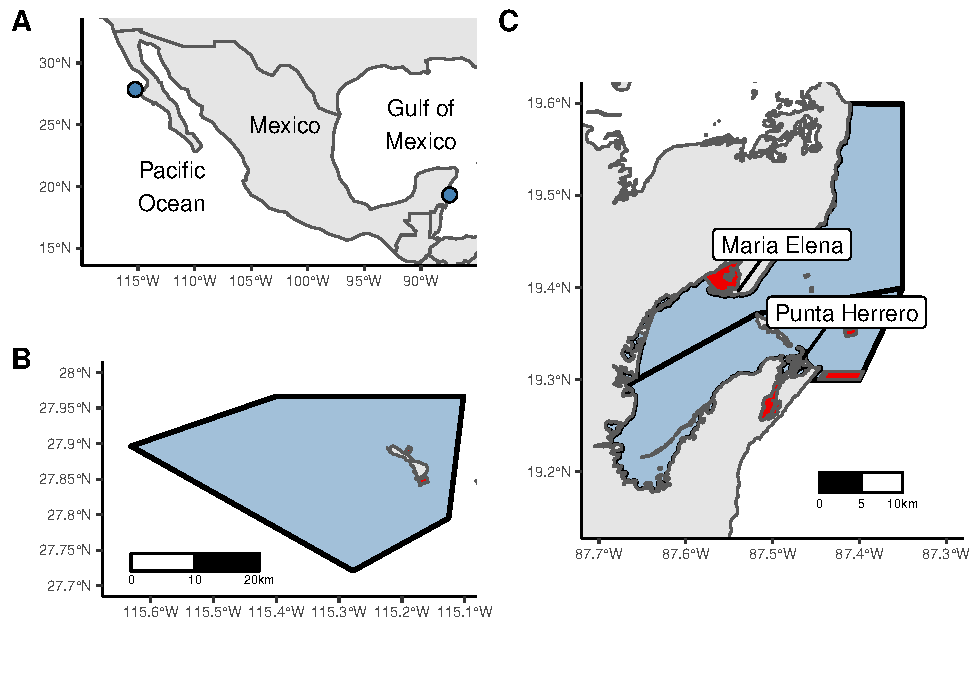
\includegraphics{Villasenor-Derbez_files/figure-latex/unnamed-chunk-1-1.pdf}
\caption{\label{fig:unnamed-chunk-1}\label{fig:map}Location of the three
coastal communities studied (A). Isla Natividad (B) is located off the
Baja California Peninsula, Maria Elena (C) and Punta Herrero (D) are
located in the Yucatan Peninsula.}
\end{figure}

\begin{table}

\caption{\label{tab:unnamed-chunk-2}\label{table:com_sum} Summary of commuity--based marine reserves by community.}
\centering
\begin{tabular}[t]{l|r|r|r|r}
\hline
Community & TURF area ($km^2$) & Reserve area ($km^2$) & Percent as reserves & Year of implementation\\
\hline
Isla Natividad & 889.5 & 1.53 & 0.1720067 & 2006\\
\hline
Maria Elena & 353.1 & 0.10 & 0.0283206 & 2012\\
\hline
Punta Herrero & 299.7 & 0.43 & 0.1434768 & 2013\\
\hline
\end{tabular}
\end{table}

Socioeconomic data come from landing receipts reported to the National
Commission for Aquaculture and Fisheries (\emph{Comisión Nacional de
Acuacultura y Pesca}; CONAPESCA). Data contain monthly lobster landings
(Kg) and value (MXP) from 2000 to 2014. This information was aggregated
by year, and economic values were adjusted by the Consumer Price Index
\citep{oecd_2017-VV} via Eq \ref{eqn:cpi}.

\begin{equation}
I_t = RI_t\times\frac{CPI_t}{CPI_T}
\label{eqn:cpi}
\end{equation}

Where \(I_t\) represents the adjusted income for year \(t\) as the
product between the reported income for that year and the ratio between
the consumer price index in that year (\(CPI_t\)) to the most recent
year's consumer price index (\(CPI_T\)).

We use a set of governance indicators to analyze the governance
structures of each cooperative \citep{leslie_2015-na}. The indicators
(Table \ref{table:gov_ind}) focus on the resource system (four
indicators), governance system (seven indicators), resource units (three
indicators) and actors (three indicators). These were collected at the
community--level from official documents used in the creation and
designation of the marine reserves
\citep{dof_website_2012,dof_website_2012} and based on the authors'
experience and knowledge of the communities.

\subsection{Data analysis}\label{data-analysis}

We evaluate the effect thar marine reserves have had on four biological
and two socioeconomic indicators (Table \ref{table:indicators}). Recall
that reserves were implemented to protect lobster and other benthic
invertebrates. However, we also contemplate fish species that are also
targeted in the off-season and might receive collateral protection from
the reserves.

\begin{table}[H]

\caption{\label{tab:unnamed-chunk-3}\label{table:indicators}List of indicators used to evaluate the effectiveness of marine reserves, grouped by category.}
\centering
\begin{tabular}[t]{l|l|l}
\hline
Category & Indicador & Units\\
\hline
Biological & Lobster density & org / $m^2$\\
\hline
Biological & Invertebrate density & org / $m^2$\\
\hline
Biological & Fish biomass & org / $m^2$\\
\hline
Biological & Fish density & org / $m^2$\\
\hline
Socioeconomic & Income from target species & M MXP\\
\hline
Socioeconomic & Landings from target species & Metric Tones\\
\hline
\end{tabular}
\end{table}

\begin{table}

\caption{\label{tab:unnamed-chunk-4}\label{table:gov_ind}Indicators used for the operationalization of the SES framework \citep{leslie_2015-na}}
\centering
\begin{tabular}[t]{>{\raggedright\arraybackslash}p{10em}|>{\raggedright\arraybackslash}p{8em}|>{\raggedright\arraybackslash}p{8em}|>{\raggedright\arraybackslash}p{8em}}
\hline
Indicator & Isla Natividad & Maria Elena & Punta Herrero\\
\hline
\textbf{Resource systems (RS)} & \textbf{} & \textbf{}\\
\hline
TURF presence & Yes & Yes & Yes\\
\hline
Type of ecosystem & Kelp Forest / Rocky Reefs & Coral Reef & Coral Reef\\
\hline
Intensity of environmental Disturbance & El nino event & Hurricanes & Hurricanes\\
\hline
Location & Island & Coastal & Coastal\\
\hline
\textbf{Governance systems (GS)} & \textbf{} & \textbf{}\\
\hline
Fishing cooperative & Yes & Yes & Yes\\
\hline
Involved actors & COBI, Stanford, REBIVI & Alianza Kanan Kay, COBI, CONANP, Coop, CONAPESCA, Oceanus, FCyRH, FHMM, & Alianza Kanan Kay, COBI, CONANP, Coop, CONAPESCA, Oceanus, FCyRH, FHMM,\\
\hline
Presence of an inter-cooperative structure & Fedecoop & Non & Non\\
\hline
Fishing Regulations & Size limits, seasonal closures, quotas & Size limits, seasonal closures & Size limits, seasonal closures\\
\hline
Enforcement technology & Boats & Boats & Land enforcement\\
\hline
MR enforcement &  &  & \\
\hline
Cooperative regulations &  &  & \\
\hline
\textbf{Resource Units (RU)} & \textbf{} & \textbf{}\\
\hline
Adult targeted species mobility & 1km & 30km & 30km\\
\hline
Targeted species longevity (years) &  &  & \\
\hline
Price of targeted species &  &  & \\
\hline
\textbf{Actors (A)} & \textbf{} & \textbf{}\\
\hline
Leadership &  &  & \\
\hline
Level of illegal fishing & 1 & 1 & 3\\
\hline
Presence of alternative livelihoods &  &  & \\
\hline
\end{tabular}
\end{table}

Biological indicators are analyzed with a difference--in--differences
analysis (Eq \ref{eqn:reg_bio}), which allows us to estimate the effect
that the reserve has on the biological indicators by comparing trends
across time and treatments
\citep{moland_2013-VP,Villasenor-Derbez_2018}. The analysis is performed
with a multiple linear regression of the form:

\begin{equation}
I_{itj} = \alpha + \gamma_{t} Year_t + \beta Zone_i + \lambda_{t} Year_t\times Zone_i + \sigma_jSpp_j + \epsilon
\label{eqn:reg_bio}
\end{equation}

Where year--fixed effects are represented by \(\gamma_{it} Year_t\), and
\(\beta Zone_i\) captures the difference between reserve (\(Zone = 1\))
and control (\(Zone = 0\)) sites. The interaction term
\(\lambda_{it} Year_t\times Zone_i\) represents represent the mean
change in the indicator inside the reserve, for year \(t\), with respect
to the first year of evaluation in the control site (See Table
\ref{table:com_sum}). When evaluating biomass and abundances, we include
species--fixed effects (\(\sigma_j\)).

Socioeconomic indicators are evaluated with a similar approach (Eq
\ref{eqn:soc_reg}). Due to data constrains, only Isla Natividad and
Maria Elena are evaluated in this case. We constructed panel-data
information with yearly (2001 - 2014) lobster landings and income of the
studied and neighbouring communities that have similar management
strategies, and belong to larger Cooperative Federtations
\citep{mccay_2017-1m,ayer_2018}. Neighbouring communities are used as
counterfacutals that allow us to control for unobserved time-invariants.
Each ``treated'' community (Isla Natividad and Maria Elena) has three
counterfactual communities.

\begin{equation}
I_i = \alpha + \gamma_{t} Year_t + \beta Treated_i + \lambda_{t} Year_t\times Treated_i + \sigma_jComm_j +\epsilon
\label{eqn:soc_reg}
\end{equation}

The model interpretation remains as for Eq \ref{eqn:reg_bio}, but in
this case the \(Treated\) dummy variable indicates if the community has
a reserve (\(Treated = 1\)) or not (\(Treated = 0\)) and
\(\sigma_jComm\) captures community-level fixed-effects. This approach
allows for a causal attribution of the observed changes to the reserve.
All model coefficients were estimated via ordinary least--squares and
heteroskedastic--robust standard errors \citep{zeileis_2004-7n}.

These regressions allows us to make a causal link between the
implementation of marine reserves and the observed trends by accounting
for temporal and spatial dynamics \citep{depalma_2018}. The effect of
the reserve is captured by the \(\lambda_t\) coefficient, and represents
the difference observed between the control site before the
implementation of the reserve and the reserve site at time \(t\) after
controlling for other time and space variations (\emph{i.e.}
\(\gamma_t\) and \(\beta\) respectively).

\section{Results}\label{results}

The following sections present the effect that marine reserves had on
each of the biological and socioeconomic indicators for each coastal
community. Results are presented in terms of the difference through time
and across sites, relative to the control site on the year of
implementation (\emph{i.e.} effect size). We also provide an overview of
the governance settings of each community, and discuss how these
dimensions might be related to the effectiveness of the reserves.

\subsection{Biological}\label{biological}

All indicators show idiosyncratic responses through time for each
community. Figure \ref{fig:indicators}A shows how lobster densities
increase inside the reserve for Isla Natividad an Punta Herrero within
the first years, but the effect is aroded through time. However, these
effects are in the order of 0.2 extra organisms \(m^{-2}\) and are not
significantly different from zero (\(p > 0.05\)). The only case when
lobster densities showed a significant positive effect (\(p < 0.1\)) was
for Isla Natividad on the sixth year (\emph{i.e.} 2012), a year after
hypoxia events described in \citet{micheli_2012-EU} caused mass
mortality of organisms. Biomass was only evaluated for fish data (Fig
\ref{fig:indicators}B), and no changes were observed (\(p > 0.1\)),
Punta Herrero even showed negative insignificant trends in the order of
0.01. Invertebrate and fish densities (\ref{fig:indicators}C-D) show
similar patterns of lack of effectiveness with effect sizes oscillating
around zero. Full tables with model coefficients are presented in the
supplementary materials (\textbf{S1 Table}, \textbf{S2 Table},
\textbf{S3 Table}).

\subsection{Socioeconomic}\label{socioeconomic}

Lobster landings and revenue were only available for Isla Natividad and
Maria Elena (Fig \ref{fig:lobsters}). For all years befor
implementation, the effect sizes are close to zero, indicating that the
control and treatment sites track each other well. However, effect sizes
do not change after the implementation of the reserve. Again, the
negative coeficient observed for Isla Natividad on year 5 correspond to
the 2011 hypoxia events. The only positive change observed in lobster
landings is for Isla Natividad in 2014 (\(p < 0.1\)). The trhee years of
post-implementation data for Maria Elena do not show a significant
effect of the reserve. Isla Natividad shows higher revenues after the
iumplementation of the reserve, as compared to the control communities.
However, these changes are also not ignificantly different and present
an increased variation. All regression coefficients for each community
and indicator are presented in \textbf{S4 Table}.

\subsection{Governance}\label{governance}

Although we have little information on the social dimension of these
fisheries, using the SES framework indicators (Table
\ref{table:gov_ind}), we can analyze the performance of each governance
system (Table \ref{table:gov_res}).

Our analysis shows that all of the systems analyzed share similarities
in their Governance system which is based on cooperatives (GS5.2.3.2),
with strong rules in use that include Operational rules (GS6.2),
Collective-choice rules (GS6.3), Constitutional rules (GS6.3), and even
Territorial use communal rights (GS6.1.4.3). However, we identified
important differences in terms of the actors, resource systems and
resource units. The value of lobster in isla natividad is higher than
the lobster sold from Punta Herrero and Maria Elena (RU4), which can
reduce the pressure on harvest. Lastly, in terms of actors, although all
communities show a high level of leadership (A5), the level of trust
(A6.1) is lower in Punta Herrero. In general, the presence and success
of conservation initiatives depends on the incentives of local
communities to maintain a healthy status of the resources they depend
upon \citep{jupiter_2017}. The enabling conditions for conservation seem
to be strongly present in all communities. Due to the clarity of access
rights and isolation, the benefits of conservation directly benefit the
members of the fishing cooperative. These conditions have favored the
development of an efficient community-based enforcement systems.

\clearpage

\begin{figure}
\centering
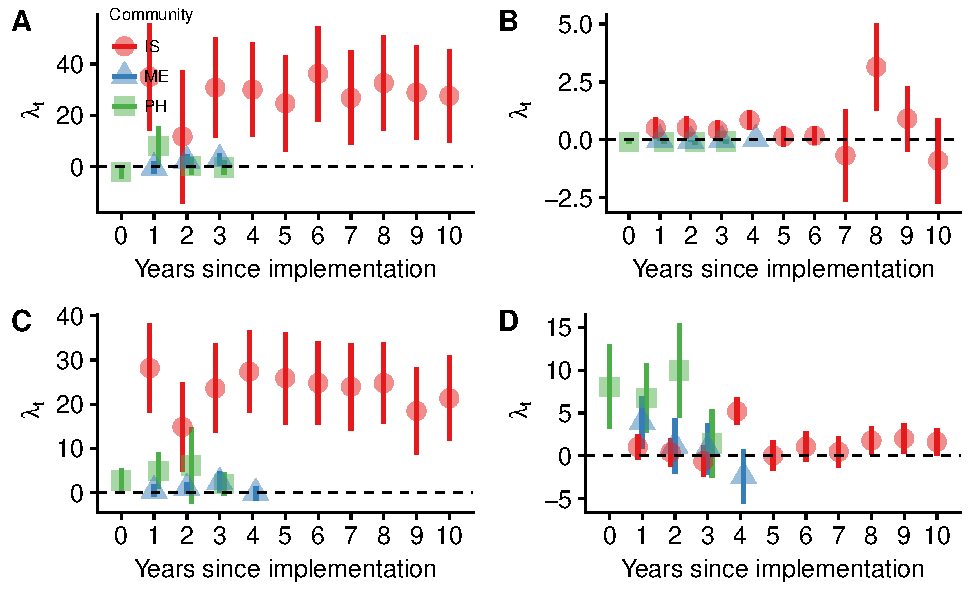
\includegraphics{Villasenor-Derbez_files/figure-latex/unnamed-chunk-5-1.pdf}
\caption{\label{fig:unnamed-chunk-5}\label{fig:indicators}Effect sizes for
marine reserves from Isla Natividad (IN; red cirlcles), Maria Elena (ME;
blue triangles), and Punta Herrero (PH; green squares) for lobster
densities (\emph{Panulirus spp}; A), fish biomass (B), invertebrate
densities (C), and fish densities (D). Plots are ordered by survey type
(left column: invertebrates; right column: fish). Points are jittered
hotizontally to avoid overplotting. Points indicate the effect size, and
errorbars standard errors. Years have been centered to year of
implementation.}
\end{figure}

\begin{figure}
\centering
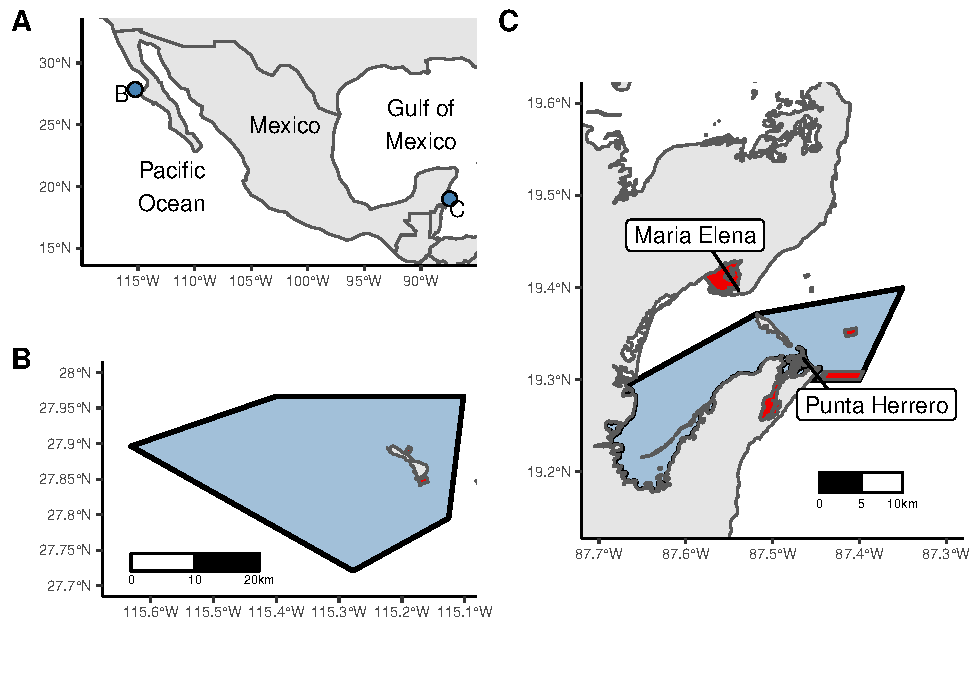
\includegraphics{Villasenor-Derbez_files/figure-latex/unnamed-chunk-7-1.pdf}
\caption{\label{fig:unnamed-chunk-7}\label{fig:lobsters}Effect sizes for
lobster catches (A) and revenues (B) in at Isla Natividad (IN; red
circles) and Maria Elena (ME; blue triangles)}
\end{figure}

\begin{table}

\caption{\label{tab:unnamed-chunk-8}\label{table:gov_res}Analysis of the fishing cooperatives based on the Social-Ecological systems framework \citep{mcginnis_2014}.}
\centering
\begin{tabular}[t]{>{\raggedright\arraybackslash}p{10em}|>{\raggedright\arraybackslash}p{10em}|l|l|l}
\hline
 & Indicator & Isla Natividad & Maria Elena & Punta Herrero\\
\hline
\textbf{Resource systems (RS)} & \textbf{} & \textbf{} & \textbf{}\\
\hline
RS2 – Clarity of system boundaries & TURF presence & High & High & High\\
\hline
RS3 – Size of resource system &  &  &  & \\
\hline
RS5 – Productivity of system & Type of ecosystem & High & High & High\\
\hline
RS7 – Predictability of system dynamics & Intensity of environmental disturbance & Low (ENSO) & High & High\\
\hline
RS9 – Location & Proximity to other communities/cities & Isolated & Not Isolated & Not Isolated\\
\hline
\textbf{Governance systems (GS)} & \textbf{} & \textbf{} & \textbf{}\\
\hline
GS1 – Government organizations & Presence of fishing cooperatives & Yes & Yes & Yes\\
\hline
GS2 – Nongovernment organizations & Involved actors & Yes & Yes & Yes\\
\hline
GS3 – Network structure & Presence of an inter-cooperative structure & Yes & No & No\\
\hline
GS4 – Property-rights systems & TURF presence & Yes & Yes & Yes\\
\hline
GS5 – Operational-choice rules & Fishing Regulations / MPA enforcement / Enforcement technolofy & Yes & Yes & Yes\\
\hline
GS6 – Collective-choice rules & Cooperative regulations & Yes & Yes & Yes\\
\hline
GS7 – Constitutional-choice rules &  &  &  & \\
\hline
\textbf{Resource units (RU)} & \textbf{} & \textbf{} & \textbf{}\\
\hline
RU1 – Resource unit mobility & Targeted species home range & Low & Medium & Medium\\
\hline
RU2 – Growth or replacement rate & Max age of targeted species & Low & Medium & Medium\\
\hline
RU4 – Economic value & Price of targeted species & high & High & high\\
\hline
\textbf{Actors (A)} & \textbf{} & \textbf{} & \textbf{}\\
\hline
A1 – Number of relevant actors &  & 98 &  & \\
\hline
A2 – Socioeconomic attributes &  &  &  & \\
\hline
A5 – Leadership/entrepreneurship & Leadership & High & High & High\\
\hline
A6 – Norms (trust-reciprocity)/social capital--- (Based on illegal fishing) & Level of illegal fishing & High & High & Low\\
\hline
A8 – Importance of resource (dependence) & Presence of alternative livelihoods & High & High & High\\
\hline
\end{tabular}
\end{table}

\clearpage

\section{Discussion}\label{discussion}

theory tells us more than 5 years are needed, so it;s not surprise for
PH and ME. But IN didnt make it either.

Our results indicated idiosyncratic biological effects of the reserves
across communities and indicators, with a combination of positive and
negative effects. However, many of these effects were not statistically
significant, indicating no effect of the reserve. The socioeconomic
indicators pertaining to landings and revenues showed little or no
change after reserve implementation. While lobster densities represent
an indicator directly tied to reserve objectives, we also evaluate other
biological indicators to test for additional effects and as a
double-check. ll indicators presented a similar pattern. The lack of
expected effectiveness poses the question, why do these communities
continue to support the reserves? While not in the main scope of this
paper, understanding the social-ecological context in which these
communities and their reserves might provide insight to answer this
question. Here, we discuss plausible explanations to lack of
effectiveness observed based on literature and our social-ecological
system analysis. We also discuss potential shortcomings in our analysis,
and provide management recommendations to improve reserve effectiveness.

Our approach to evaluate the temporal and spatial changes of each
indicator provides a more robust measure of reserve effectiveness. Some
works have solely focused on an inside-outside comparison of indicators
\citep{guidetti_2014-8Z,friedlander_2017-oI,rodriguez_2017-PD}, which do
not address temporal variability \citep{depalma_2018}. Other works have
compared the trend observed within a reserve through time
\citep{betti_2017-lq}, which cannot distinguish between the temporal
trends in a reserve and the entire system \citep{depalma_2018}. By
accounting for trends between sites and through time, we can control for
time and space dynamics, and provide a better identification of the
effect

Age, isolation, and enforcement are important factors influencing
effectiveness of a marine reserve \citep{edgar_2014-UO}. Isla Natividad
has the oldest reserve, is fairly isolated, and has a well-established
community-based enforcement system. Neighbouring fishing communities are
known to be well organized with successful resource management of their
resources \citep{mccay_2017-1m,mccay_2014-CN}. Maria Elena and Punta
Herrero are relatively young reserves (Table \ref{table:com_sum}). With
the age, relative isolation, and enforcement level of these reserves,
one would expect to observe effectiveness. However, another key feature
of effective MRs is size \citep{edgar_2014-UO}; the lack of
effectiveness is perhaps attributed to the reserves being too small
\ref{table:com_sum}. Furthermore, perturbations that do not distinguish
reserve boundaries, such as the environmental variability observed in
Isla Natividad can also hinder effectiveness. The possibility of
increasing reserve size or merging existing networks into a larger
reserve should be evaluated.

Our analysis of landings and revenues does not identify detectable
changes in these indicators. However, previous research has shown that
reserves in Isla Natividad yield fishery benefits for the abalone
fishery \citep{rossetto_2015-V0}. Abalone are sesile invertebrates with
less mobility (compared to lobsters), and thus current reserve size
might not be enough for lobster's range of mobility even when accounting
for reserve age in Isla Natividad. Other community-based marine reserves
in tropical ecosystems have taken up to six years to show a spillover
effect \citep{dasilva_2015-zX}. Reserves in Maria Elena and Punta
Herrero are relatively small and young, and may need more time for
abundances to increase enough to export larvae or adult organisms.

A second explanation lies on the the mismatch of objectives during the
design process. The Project description (\emph{Estudios Técnicos
Justificativos}) of each MR provides little information about the
followed design guidelines. However, all reserves had to be approved by
the community members. Depending on the communities' capacity to look
for longterm benefits, many communities may favor implementation of
reserves on sites that represent a low fishing cost. As a consequence,
the marine reserve have low impacts in reducng the fishing effort.
Having small reserves in areas that do not compromise fishing profits
might explain why this communities still support their reserves.

Although our case studies fulfilled the social requirements for
effective marine reserves (``high enforcement, presence of a management
plan, fisher engagement in management, and promotion of sustainable
fishing''; \citet{difranco_2016-Xw}), our results show that proper
reserve design is crucial for effective marine reserves. The
social-ecological systems framework allowed a systematic diganosis and
compare all the different case studies, allowing us to identify and
tease appart possible explanations \citep{basurto_2013-oq}.

\section*{Conflict of Interest Statement}

The authors declare that the research was conducted in the absence of
any commercial or financial relationships that could be construed as a
potential conflict of interest.

\section*{Author Contributions}

JC and EA analyzed and interpreted data, discussed the results, and
wrote the manuscript. AS, SF and JT edited the manuscript and discussed
the results.

\section*{Funding}

JCVD CONACyT + LAFF ASC SF JT

\section*{Acknowledgments}

The authors wish to acknowledge Arturo Hernández and Imelda Amador for
contributions on the governance data, as well as pre-processing
biological data. This study would have not been possible without the
effort by members of the communities here mentioned, who collected the
biological data.

\section*{Supplemental Data}

\href{http://home.frontiersin.org/about/author-guidelines#SupplementaryMaterial}{Supplementary Material}
should be uploaded separately on submission, if there are Supplementary
Figures, please include the caption in the same file as the figure.
LaTeX Supplementary Material templates can be found in the Frontiers
LaTeX folder

\paragraph*{S1 Figure}
\label{S1_Figure}

Timeseries of indicators for IN

\paragraph*{S2 Figure}
\label{S2_Figure}

Timeseries of indicators for ME

\paragraph*{S3 Figure}
\label{S3_Figure}

Timeseries of indicators for PH

\paragraph*{S1 Table}
\label{S1_Table}

Coefficient estimates for Isla Natividad

\paragraph*{S2 Table}
\label{S2_Table}

Coefficient estimates for Maria Elena

\paragraph*{S3 Table}
\label{S3_Table}

Coefficient estimates for Punta Herrero

\bibliographystyle{frontiersinSCNS_ENG_HUMS}\bibliography{references}

\section*{Figure captions}



\end{document}
